\documentclass[tikz,margin=2mm]{standalone}
\usetikzlibrary{positioning, arrows.meta}
\usepackage{bm}

\begin{document}

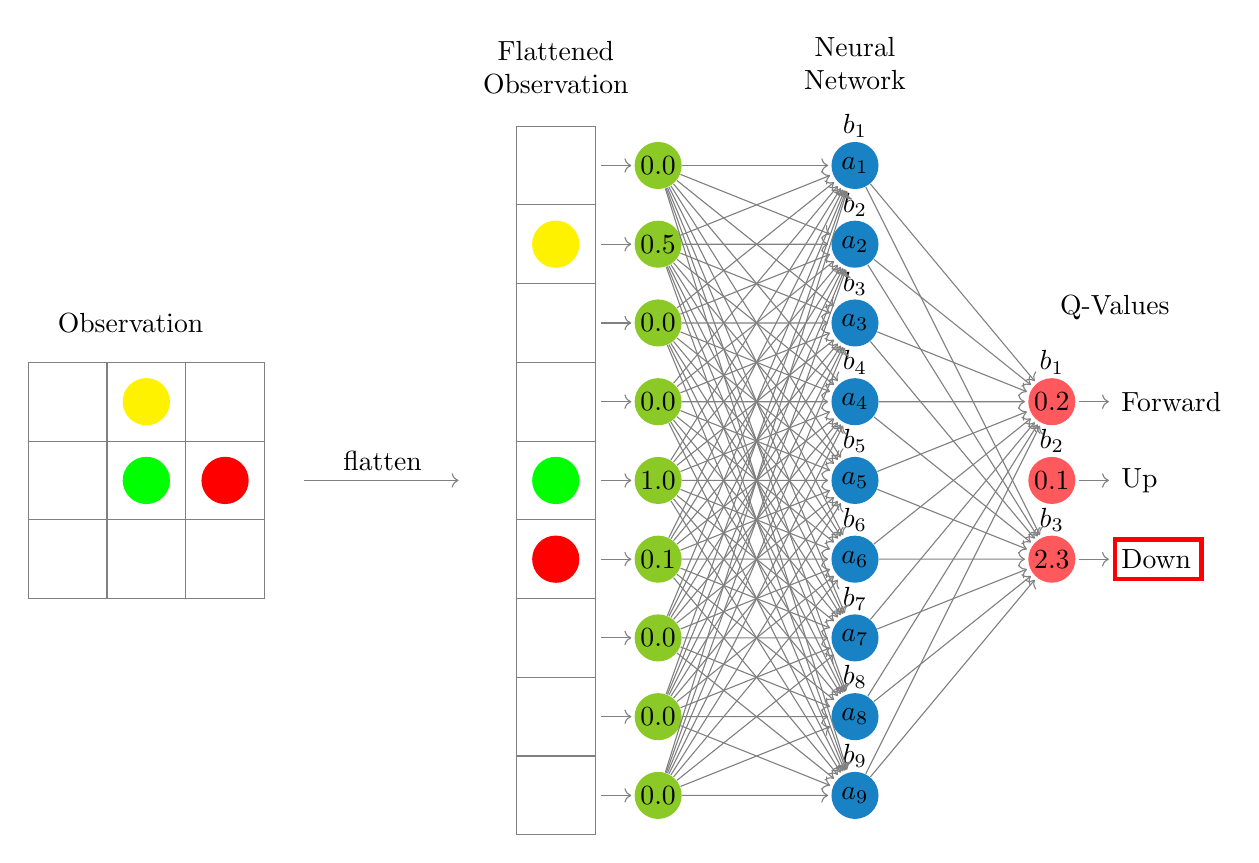
\begin{tikzpicture}[shorten >=1pt,->,draw=black!50, node distance=\layersep]
    \definecolor{inp}{HTML}{8ac926}
    \definecolor{hid}{HTML}{1982c4}
    \definecolor{outp}{HTML}{ff595e}
    \newcommand{\layersep}{2.5cm}
    \tikzstyle{every pin edge}=[<-,shorten <=1pt]
    \tikzstyle{neuron}=[circle,fill=black!25,minimum size=17pt,inner sep=0pt]
    \tikzstyle{input neuron}=[neuron, fill=inp];
    \tikzstyle{output neuron}=[neuron, fill=outp];
    \tikzstyle{hidden neuron}=[neuron, fill=hid];
    \tikzstyle{annot} = [text width=6em, text centered]

    % Draw the 3x3 grid
    \foreach \x in {-8,...,-6} {
        \foreach \y in {-6.5,...,-4.5} {
            \draw (\x,\y) rectangle ++(1,1); % Draw gridlines
        }
    }
    \foreach \i/\j/\k in {red/-6/-5, green/-7/-5, yellow/-7/-4} {
        \fill[\i] (\j+0.5,\k) circle (0.3); % Fill specific cells with different colors
    }

    % Draw the flattened grid
    \foreach \x in {-9.5,...,-1.5} {
        \draw (-1.8,\x) rectangle ++(1,1); % Draw gridlines
    }

    % Draw the particles in the flattened grid
    \foreach \i/\j/\k in {red/-1.8/-6.5, green/-1.8/-5.5, yellow/-1.8/-2.5} {
        \fill[\i] (\j+0.5,\k+0.5) circle (0.3); % Fill specific cells with different colors
    }

    % Draw the arrow from the grid to the flattened grid
    \draw[->] (-4.5,-5) -- (-2.5,-5) node[midway,above] {flatten};

    % Draw the input layer nodes
    \foreach \name / \y in {1/0.0, 2/0.5, 3/0.0, 4/0.0, 5/1.0, 6/0.1, 7/0.0, 8/0.0, 9/0.0}
    \node[input neuron, pin=left:] (I-\name) at (0,-\name) {\y};

    % Draw the hidden layer nodes
    \foreach \name / \y in {1,...,9}
    \path[yshift=0cm]
    node[hidden neuron] (H-\name) at (\layersep,-\y cm) {$a_{\y}$}
    node[annot,above of=H-\name, node distance=0.5cm] (hl) {$b_{\y}$};

    % Draw the output layer node
    \foreach \txt / \y / \qval in {Forward/1/0.2,Up/2/0.1,Down/3/2.3}
    \path[yshift=-3cm]
    node[output neuron,pin={[pin edge={->}]right:\txt}] (O-\y) at (2*\layersep,-\y) {\qval}
    node[annot,above of=O-\y, node distance=0.5cm] (hl) {$b_{\y}$};

    % red box around the Down label
    \draw[red,ultra thick] (5.8,-6.25) rectangle ++(1.1,0.5);

    % Connect every node in the input layer with every node in the
    % hidden layer.
    \foreach \source in {1,...,9}
    \foreach \dest in {1,...,9}
    \path (I-\source) edge (H-\dest);

    % Connect every node in the hidden layer with the output layer
    \foreach \source in {1,...,9}
    \foreach \dest in {1,3}
    \path (H-\source) edge (O-\dest);

    % Annotate the network
    \node[annot,above of=H-1, node distance=1.3cm] (hl) {Neural Network};
    % Annotate the 3x3 grid
    \node[annot] at (-6.7,-3) {Observation};
    % Annotate the flattened grid
    \node[annot] at (-1.3,0.25) {Flattened Observation};
    % Annotate the Q values
    \node[annot] at (5.8,-2.8) {Q-Values};
\end{tikzpicture}

\end{document}